\section{Grundlagen} \label{sec:Grundlagen}

\subsection{Anlagenübersicht}
\begin{figure}[H]
   \centering
   \fbox{\includegraphics[width=0.8\textwidth]{Bilder/1. Grundlagen/(1.1) Anlagenübersicht.png}}
   \caption[Anlagenübersicht]{Anlagenübersicht}
   \label{fig:Bild1.1}
\end{figure}

\begin{figure}[H]
   \centering
   \fbox{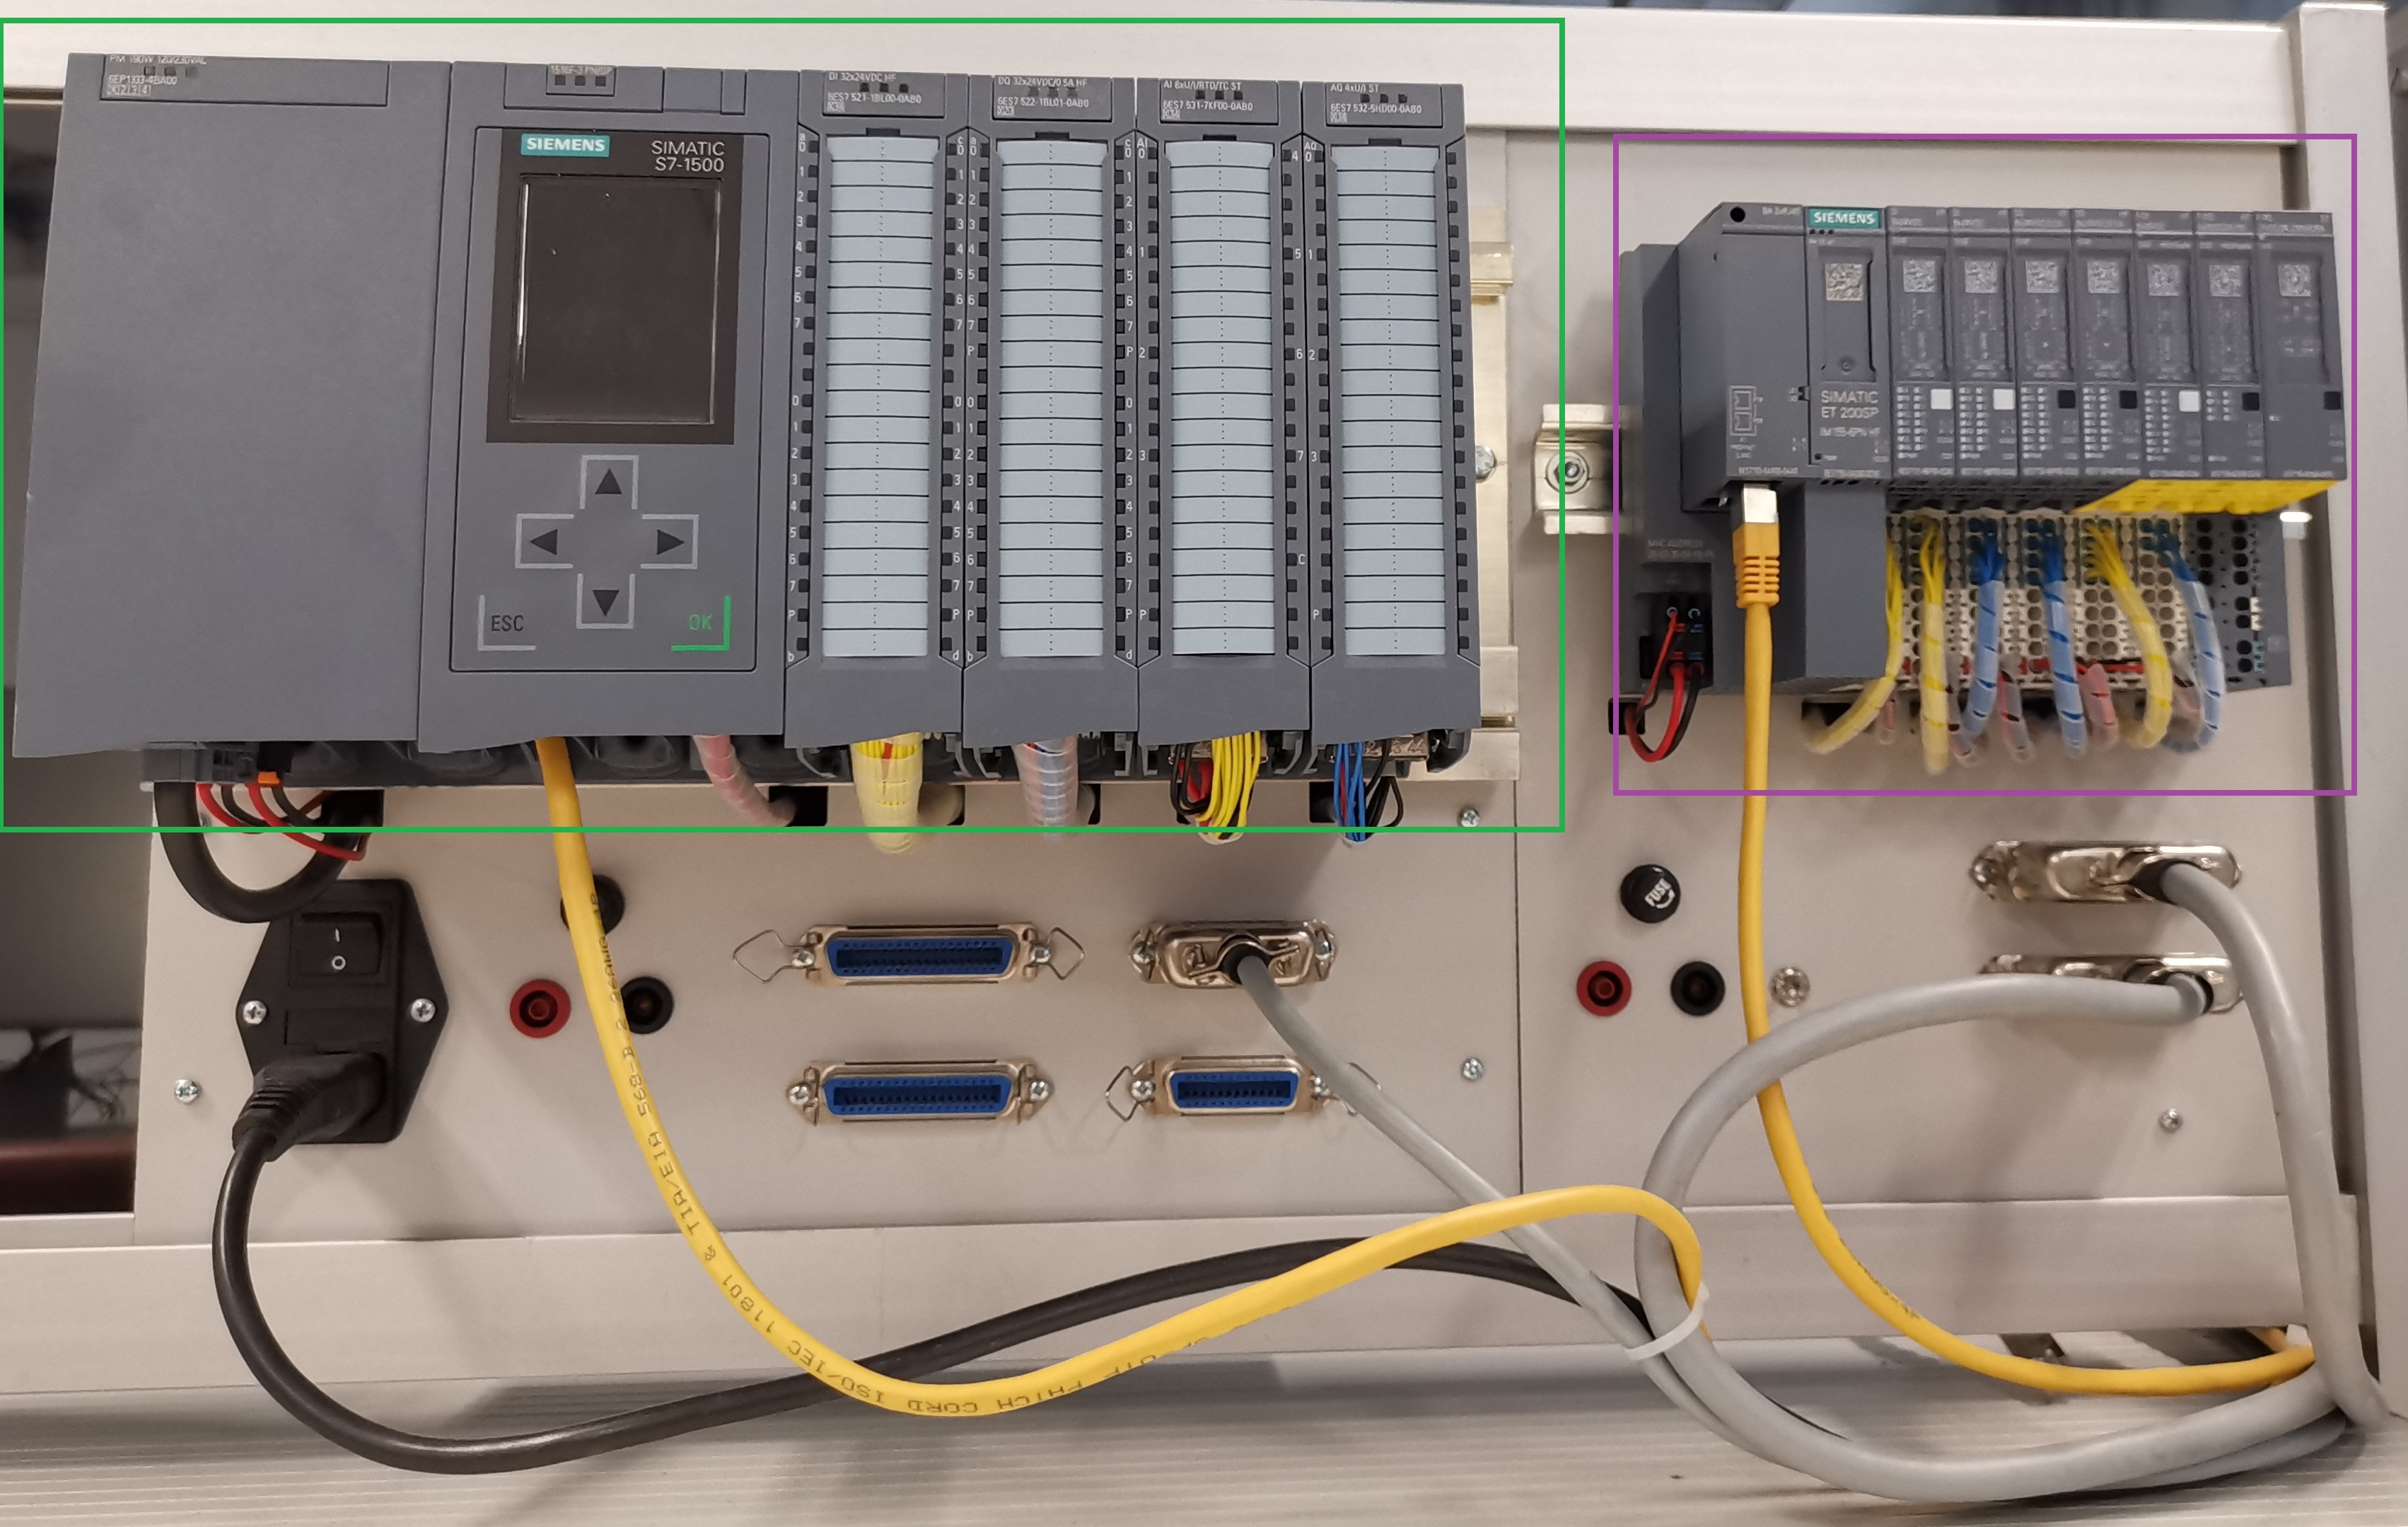
\includegraphics[width=0.8\textwidth]{Bilder/1. Grundlagen/(1.2) Reale Anlage.jpg}}
   \caption[Reale Anlage]{Reale Anlage (links: S7-1500; rechts: ET 200SP)}
   \label{fig:Bild1.2}
\end{figure}

\subsection{PROFINET-Gerätenamen und IP-Adressen im Raum WH G-420}
\begin{figure}[H]
    \centering
    \begin{tikzpicture}[framed][domain=0:0]
        % Umrandung zeichnen
        \draw[black, very thick] (0,0) rectangle (15,17);
        
        % Eingangstür zeichnen
        \draw[black, very thick](15,0.7) -- (13, 0.7);
        \draw[grey, very thin] (15,2.7) arc (90:180:2);
        
        % Tür zum Büro
        \draw[black, very thick](9, 17) -- (9, 15);
        \draw[grey, very thin] (11, 17) arc (0:-90:2);
        
        % Tafel
        \draw[black, fill = black] (5.5, 0.3) rectangle (9.5, 0.4);
        \draw[black, fill = black] (9.5,0.3) -- (11.5, 1) -- ++(109.29:0.1cm) -- ++(199.29:2.12cm) -- ++(289.29:0.1cm);
        \draw[black, fill = black] (5.5, 0.3) -- (3.5, 1) -- ++(70.71:0.1cm) -- ++(-19.29:2.12cm) -- ++(-109.29:0.1cm);
        
        % Arbeitsplätze Wand
        \draw[black, dashed] (11.3, 2.9) rectangle (14.8, 5.7);
        \draw[black, dashed] (11.3, 5.9) rectangle (14.8, 8.7);
        \draw[black, dashed] (11.3, 8.9) rectangle (14.8, 11.7);
        \draw[black, dashed] (11.3, 11.9) rectangle (14.8, 14.7);
        
        % Arbeitsplätze Fenster
        \draw[black, dashed] (0.2, 2.9) rectangle (3.7, 5.7);
        \draw[black, dashed] (0.2, 5.9) rectangle (3.7, 8.7);
        \draw[black, dashed] (0.2, 8.9) rectangle (3.7, 11.7);
        \draw[black, dashed] (0.2, 11.9) rectangle (3.7, 14.7);
        
        % Arbeitsplätze Gang
        \draw[black, dashed] (3.9, 2.9) rectangle (7.4, 5.7);
        \draw[black, dashed] (3.9, 5.9) rectangle (7.4, 8.7);
        \draw[black, dashed] (3.9, 8.9) rectangle (7.4, 11.7);
        \draw[black, dashed] (3.9, 11.9) rectangle (7.4, 14.7);
        
        % Raum
        \node[font=\bfseries, scale = 1] at (2, 16.5) {Raum WH G-420};
        
        % Subnetz-Text
        \node[scale = 0.8] at (1.9, 16) {Subnetz: 255.255.255.0};
        
        % Gerätenamen PC's & IP-Adressen Fenster
        \node[font=\bfseries, scale = 0.8] at (1.85, 14.4) {FB1-G420-04};
        \node[scale = 0.75] at (1.85, 14) {192.168.1.14};
        \node[font=\bfseries, scale = 0.8] at (1.85, 13.5) {s7-1500-fenster-4};
        \node[scale = 0.75] at (1.85, 13.1) {192.168.1.114};
        \node[font=\bfseries, scale = 0.8] at (1.85, 12.6) {et-200-fenster-4};
        \node[scale = 0.75] at (1.85, 12.2) {192.168.1.134};
        
        \node[font=\bfseries, scale = 0.8] at (1.85, 11.4) {FB1-G420-03};
        \node[scale = 0.75] at (1.85, 11) {192.168.1.13};
        \node[font=\bfseries, scale = 0.8] at (1.85, 10.5) {s7-1500-fenster-3};
        \node[scale = 0.75] at (1.85, 10.1) {192.168.1.113};
        \node[font=\bfseries, scale = 0.8] at (1.85, 9.6) {et-200-fenster-3};
        \node[scale = 0.75] at (1.85, 9.2) {192.168.1.133};
        
        \node[font=\bfseries, scale = 0.8] at (1.85, 8.4) {FB1-G420-02};
        \node[scale = 0.75] at (1.85, 8) {192.168.1.12};
        \node[font=\bfseries, scale = 0.8] at (1.85, 7.5) {s7-1500-fenster-2};
        \node[scale = 0.75] at (1.85, 7.1) {192.168.1.112};
        \node[font=\bfseries, scale = 0.8] at (1.85, 6.6) {et-200-fenster-2};
        \node[scale = 0.75] at (1.85, 6.2) {192.168.1.132};
        
        \node[font=\bfseries, scale = 0.8] at (1.85, 5.4) {FB1-G420-01};
        \node[scale = 0.75] at (1.85, 5) {192.168.1.11};
        \node[font=\bfseries, scale = 0.8] at (1.85, 4.5) {s7-1500-fenster-1};
        \node[scale = 0.75] at (1.85, 4.1) {192.168.1.111};
        \node[font=\bfseries, scale = 0.8] at (1.85, 3.6) {et-200-fenster-1};
        \node[scale = 0.75] at (1.85, 3.2) {192.168.1.131};
        
        % Gerätenamen PC's & IP-Adressen Gang
        \node[font=\bfseries, scale = 0.8] at (5.6, 14.4) {FB1-G420-08};
        \node[scale = 0.75] at (5.6, 14) {192.168.1.18};
        \node[font=\bfseries, scale = 0.8] at (5.6, 13.5) {s7-1500-gang-4};
        \node[scale = 0.75] at (5.6, 13.1) {192.168.1.118};
        \node[font=\bfseries, scale = 0.8] at (5.6, 12.6) {et-200-gang-4};
        \node[scale = 0.75] at (5.6, 12.2) {192.168.1.138};
        
        \node[font=\bfseries, scale = 0.8] at (5.6, 11.4) {FB1-G420-07};
        \node[scale = 0.75] at (5.6, 11) {192.168.1.17};
        \node[font=\bfseries, scale = 0.8] at (5.6, 10.5) {s7-1500-gang-3};
        \node[scale = 0.75] at (5.6, 10.1) {192.168.1.117};
        \node[font=\bfseries, scale = 0.8] at (5.6, 9.6) {et-200-gang-3};
        \node[scale = 0.75] at (5.6, 9.2) {192.168.1.137};
        
        \node[font=\bfseries, scale = 0.8] at (5.6, 8.4) {FB1-G420-06};
        \node[scale = 0.75] at (5.6, 8) {192.168.1.16};
        \node[font=\bfseries, scale = 0.8] at (5.6, 7.5) {s7-1500-gang-2};
        \node[scale = 0.75] at (5.6, 7.1) {192.168.1.116};
        \node[font=\bfseries, scale = 0.8] at (5.6, 6.6) {et-200-gang-2};
        \node[scale = 0.75] at (5.6, 6.2) {192.168.1.136};
        
        \node[font=\bfseries, scale = 0.8] at (5.6, 5.4) {FB1-G420-05};
        \node[scale = 0.75] at (5.6, 5) {192.168.1.15};
        \node[font=\bfseries, scale = 0.8] at (5.6, 4.5) {s7-1500-gang-1};
        \node[scale = 0.75] at (5.6, 4.1) {192.168.1.115};
        \node[font=\bfseries, scale = 0.8] at (5.6, 3.6) {et-200-gang-1};
        \node[scale = 0.75] at (5.6, 3.2) {192.168.1.135};
        
        % Gerätenamen PC's & IP-Adressen Wand
        \node[font=\bfseries, scale = 0.8] at (13, 14.4) {FB1-G420-12};
        \node[scale = 0.75] at (13, 14) {192.168.1.22};
        \node[font=\bfseries, scale = 0.8] at (13, 13.5) {s7-1500-wand-4};
        \node[scale = 0.75] at (13, 13.1) {192.168.1.122};
        \node[font=\bfseries, scale = 0.8] at (13, 12.6) {et-200-wand-4};
        \node[scale = 0.75] at (13, 12.2) {192.168.1.142};
        
        \node[font=\bfseries, scale = 0.8] at (13, 11.4) {FB1-G420-11};
        \node[scale = 0.75] at (13, 11) {192.168.1.21};
        \node[font=\bfseries, scale = 0.8] at (13, 10.5) {s7-1500-wand-3};
        \node[scale = 0.75] at (13, 10.1) {192.168.1.121};
        \node[font=\bfseries, scale = 0.8] at (13, 9.6) {et-200-wand-3};
        \node[scale = 0.75] at (13, 9.2) {192.168.1.141};
        
        \node[font=\bfseries, scale = 0.8] at (13, 8.4) {FB1-G420-10};
        \node[scale = 0.75] at (13, 8) {192.168.1.20};
        \node[font=\bfseries, scale = 0.8] at (13, 7.5) {s7-1500-wand-2};
        \node[scale = 0.75] at (13, 7.1) {192.168.1.120};
        \node[font=\bfseries, scale = 0.8] at (13, 6.6) {et-200-wand-2};
        \node[scale = 0.75] at (13, 6.2) {192.168.1.140};
        
        \node[font=\bfseries, scale = 0.8] at (13, 5.4) {FB1-G420-09};
        \node[scale = 0.75] at (13, 5) {192.168.1.19};
        \node[font=\bfseries, scale = 0.8] at (13, 4.5) {s7-1500-wand-1};
        \node[scale = 0.75] at (13, 4.1) {192.168.1.119};
        \node[font=\bfseries, scale = 0.8] at (13, 3.6) {et-200-wand-1};
        \node[scale = 0.75] at (13, 3.2) {192.168.1.139};
    \end{tikzpicture}
    \caption[IP-Adressen und PROFINET-Gerätenamen im Raum WH G-420]{IP-Adressen und PROFINET-Gerätenamen im Raum WH G-420}
    \label{fig:Bild1.3}
\end{figure}